\documentclass{standalone}
\usepackage{pgfplots}
\pgfplotsset{compat=1.18}
\usepgfplotslibrary{fillbetween}

\begin{document}
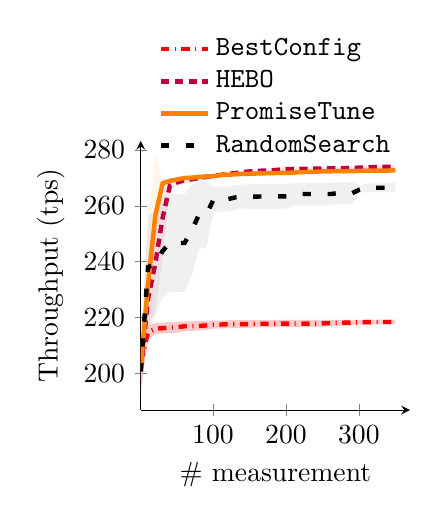
\begin{tikzpicture}
    \begin{axis}[
      axis x line  = bottom,
      axis y line  = left,
      width=5cm, height=5cm, 
      xlabel={\# measurement},
      ylabel={Throughput (tps)},
      xmin=1.0000, xmax=370.0000,
      ymin=186.9695, ymax=283.1976,
      legend cell align=left,
      legend columns=1,
      legend style={
        draw=none, fill=none,
        at={(0.98,0.9)}, anchor=south east,
        legend cell align=left
      }
    ]


\addplot[
    red,
    dashdotted,
    ultra thick, forget plot
] coordinates {
(1.0000, 204.3271) (11.0000, 214.7604) (21.0000, 216.0288) (31.0000, 216.2480) (41.0000, 216.4655) (51.0000, 216.5626) (61.0000, 216.9475) (71.0000, 217.0066) (81.0000, 217.0566) (91.0000, 217.2264) (101.0000, 217.4884) (111.0000, 217.5533) (121.0000, 217.6604) (131.0000, 217.6701) (141.0000, 217.6848) (151.0000, 217.7499) (161.0000, 217.8228) (171.0000, 217.8235) (181.0000, 217.8496) (191.0000, 217.8856) (201.0000, 217.8895) (211.0000, 217.8895) (221.0000, 217.8912) (231.0000, 217.8918) (241.0000, 217.9027) (251.0000, 217.9852) (261.0000, 218.0299) (271.0000, 218.1356) (281.0000, 218.2095) (291.0000, 218.2519) (301.0000, 218.3725) (311.0000, 218.4316) (321.0000, 218.4536) (331.0000, 218.4545) (341.0000, 218.4640) (350.0000, 218.4771)
}; 
\addlegendentry{\texttt{BestConfig}}

\addplot[
name path=upper0,
draw=none, forget plot
] coordinates {
(1.0000, 214.2753) (11.0000, 217.1783) (21.0000, 218.1051) (31.0000, 218.1897) (41.0000, 218.3900) (51.0000, 218.5488) (61.0000, 218.6915) (71.0000, 218.7075) (81.0000, 218.7571) (91.0000, 218.8064) (101.0000, 218.9325) (111.0000, 218.9925) (121.0000, 219.0850) (131.0000, 219.0943) (141.0000, 219.1022) (151.0000, 219.1033) (161.0000, 219.1228) (171.0000, 219.1225) (181.0000, 219.1408) (191.0000, 219.1795) (201.0000, 219.1896) (211.0000, 219.1896) (221.0000, 219.1915) (231.0000, 219.1921) (241.0000, 219.2043) (251.0000, 219.1708) (261.0000, 219.1731) (271.0000, 219.2516) (281.0000, 219.2116) (291.0000, 219.2007) (301.0000, 219.2283) (311.0000, 219.2631) (321.0000, 219.2836) (331.0000, 219.2848) (341.0000, 219.2982) (350.0000, 219.3115)
}; 

\addplot[
name path=lower0,
draw=none, forget plot
] coordinates {
(1.0000, 194.3788) (11.0000, 212.3424) (21.0000, 213.9525) (31.0000, 214.3063) (41.0000, 214.5411) (51.0000, 214.5765) (61.0000, 215.2036) (71.0000, 215.3057) (81.0000, 215.3560) (91.0000, 215.6464) (101.0000, 216.0443) (111.0000, 216.1140) (121.0000, 216.2358) (131.0000, 216.2460) (141.0000, 216.2674) (151.0000, 216.3964) (161.0000, 216.5228) (171.0000, 216.5245) (181.0000, 216.5585) (191.0000, 216.5917) (201.0000, 216.5895) (211.0000, 216.5895) (221.0000, 216.5908) (231.0000, 216.5914) (241.0000, 216.6011) (251.0000, 216.7996) (261.0000, 216.8867) (271.0000, 217.0195) (281.0000, 217.2074) (291.0000, 217.3031) (301.0000, 217.5167) (311.0000, 217.6000) (321.0000, 217.6235) (331.0000, 217.6241) (341.0000, 217.6298) (350.0000, 217.6427)
}; 

% ========= file shading =========
\addplot[
    red!70,
    fill opacity=0.30, forget plot
] fill between[
    of=upper0 and lower0,
];


\addplot[
    purple,
    densely dashed,
    ultra thick, forget plot
] coordinates {
(1.0000, 201.2703) (11.0000, 226.8445) (21.0000, 239.4067) (31.0000, 255.7209) (41.0000, 267.2971) (51.0000, 268.3639) (61.0000, 269.1891) (71.0000, 269.5041) (81.0000, 269.9720) (91.0000, 270.2971) (101.0000, 270.7131) (111.0000, 271.0477) (121.0000, 271.4642) (131.0000, 271.6724) (141.0000, 272.0675) (151.0000, 272.3237) (161.0000, 272.4720) (171.0000, 272.6073) (181.0000, 272.7122) (191.0000, 272.9130) (201.0000, 273.1020) (211.0000, 273.1860) (221.0000, 273.2000) (231.0000, 273.2327) (241.0000, 273.2994) (251.0000, 273.3549) (261.0000, 273.3873) (271.0000, 273.4450) (281.0000, 273.5134) (291.0000, 273.5394) (301.0000, 273.6410) (311.0000, 273.7214) (321.0000, 273.8127) (331.0000, 273.9200) (341.0000, 273.9571) (350.0000, 274.0237)
}; 
\addlegendentry{\texttt{HEBO}}

\addplot[
name path=upper1,
draw=none, forget plot
] coordinates {
(1.0000, 209.7800) (11.0000, 240.3662) (21.0000, 255.9289) (31.0000, 269.8328) (41.0000, 269.1367) (51.0000, 269.7383) (61.0000, 270.3647) (71.0000, 270.6975) (81.0000, 271.0509) (91.0000, 271.2577) (101.0000, 271.5524) (111.0000, 271.8343) (121.0000, 272.0830) (131.0000, 272.1194) (141.0000, 272.7250) (151.0000, 273.0035) (161.0000, 273.0862) (171.0000, 273.2388) (181.0000, 273.3918) (191.0000, 273.4671) (201.0000, 273.6414) (211.0000, 273.8268) (221.0000, 273.8374) (231.0000, 273.8734) (241.0000, 273.8428) (251.0000, 273.8886) (261.0000, 273.9192) (271.0000, 273.9775) (281.0000, 274.0243) (291.0000, 274.0850) (301.0000, 274.1910) (311.0000, 274.2383) (321.0000, 274.2923) (331.0000, 274.3736) (341.0000, 274.4054) (350.0000, 274.5370)
}; 

\addplot[
name path=lower1,
draw=none, forget plot
] coordinates {
(1.0000, 192.7606) (11.0000, 213.3227) (21.0000, 222.8845) (31.0000, 241.6090) (41.0000, 265.4575) (51.0000, 266.9896) (61.0000, 268.0135) (71.0000, 268.3107) (81.0000, 268.8931) (91.0000, 269.3364) (101.0000, 269.8738) (111.0000, 270.2610) (121.0000, 270.8454) (131.0000, 271.2253) (141.0000, 271.4100) (151.0000, 271.6440) (161.0000, 271.8578) (171.0000, 271.9758) (181.0000, 272.0326) (191.0000, 272.3588) (201.0000, 272.5625) (211.0000, 272.5453) (221.0000, 272.5626) (231.0000, 272.5920) (241.0000, 272.7559) (251.0000, 272.8211) (261.0000, 272.8553) (271.0000, 272.9124) (281.0000, 273.0026) (291.0000, 272.9938) (301.0000, 273.0910) (311.0000, 273.2046) (321.0000, 273.3331) (331.0000, 273.4665) (341.0000, 273.5089) (350.0000, 273.5105)
}; 

% ========= file shading =========
\addplot[
    purple!30,
    fill opacity=0.30, forget plot
] fill between[
    of=upper1 and lower1,
];


\addplot[
    orange,
    solid,
    ultra thick, forget plot
] coordinates {
(1.0000, 202.2027) (11.0000, 232.1878) (21.0000, 256.5710) (31.0000, 268.0235) (41.0000, 268.9006) (51.0000, 269.4299) (61.0000, 269.9337) (71.0000, 270.0407) (81.0000, 270.3077) (91.0000, 270.5054) (101.0000, 270.5702) (111.0000, 271.0019) (121.0000, 271.0872) (131.0000, 271.2508) (141.0000, 271.4004) (151.0000, 271.4417) (161.0000, 271.5603) (171.0000, 271.6133) (181.0000, 271.6666) (191.0000, 271.7555) (201.0000, 271.7663) (211.0000, 271.8962) (221.0000, 272.0457) (231.0000, 272.1104) (241.0000, 272.1728) (251.0000, 272.3215) (261.0000, 272.3292) (271.0000, 272.3684) (281.0000, 272.3753) (291.0000, 272.3776) (301.0000, 272.5143) (311.0000, 272.5939) (321.0000, 272.5939) (331.0000, 272.5939) (341.0000, 272.5958) (350.0000, 272.6782)
}; 
\addlegendentry{\texttt{PromiseTune}}

\addplot[
name path=upper2,
draw=none, forget plot
] coordinates {
(1.0000, 207.4184) (11.0000, 254.3555) (21.0000, 278.1562) (31.0000, 269.1785) (41.0000, 269.7881) (51.0000, 270.0260) (61.0000, 270.8981) (71.0000, 270.9162) (81.0000, 271.2153) (91.0000, 271.3665) (101.0000, 271.3191) (111.0000, 271.7481) (121.0000, 271.7578) (131.0000, 271.8346) (141.0000, 272.0522) (151.0000, 272.0148) (161.0000, 271.9985) (171.0000, 272.0115) (181.0000, 272.0802) (191.0000, 272.0582) (201.0000, 272.0730) (211.0000, 272.2103) (221.0000, 272.3970) (231.0000, 272.5057) (241.0000, 272.5663) (251.0000, 272.6677) (261.0000, 272.6753) (271.0000, 272.7237) (281.0000, 272.7310) (291.0000, 272.7317) (301.0000, 272.9942) (311.0000, 273.0672) (321.0000, 273.0672) (331.0000, 273.0672) (341.0000, 273.0678) (350.0000, 273.0565)
}; 

\addplot[
name path=lower2,
draw=none, forget plot
] coordinates {
(1.0000, 196.9869) (11.0000, 210.0201) (21.0000, 234.9857) (31.0000, 266.8684) (41.0000, 268.0131) (51.0000, 268.8337) (61.0000, 268.9693) (71.0000, 269.1652) (81.0000, 269.4002) (91.0000, 269.6442) (101.0000, 269.8212) (111.0000, 270.2557) (121.0000, 270.4165) (131.0000, 270.6671) (141.0000, 270.7486) (151.0000, 270.8686) (161.0000, 271.1221) (171.0000, 271.2151) (181.0000, 271.2529) (191.0000, 271.4528) (201.0000, 271.4596) (211.0000, 271.5821) (221.0000, 271.6945) (231.0000, 271.7151) (241.0000, 271.7794) (251.0000, 271.9754) (261.0000, 271.9832) (271.0000, 272.0132) (281.0000, 272.0195) (291.0000, 272.0234) (301.0000, 272.0344) (311.0000, 272.1206) (321.0000, 272.1206) (331.0000, 272.1206) (341.0000, 272.1238) (350.0000, 272.2999)
}; 

% ========= file shading =========
\addplot[
    orange!30,
    fill opacity=0.30, forget plot
] fill between[
    of=upper2 and lower2,
];


\addplot[
    black,
    loosely dashed,
    ultra thick, forget plot
] coordinates {
(1.0000, 200.7812) (11.0000, 238.1029) (21.0000, 239.0653) (31.0000, 243.8922) (41.0000, 246.6896) (51.0000, 246.6896) (61.0000, 246.6896) (71.0000, 251.2510) (81.0000, 256.9562) (91.0000, 256.9562) (101.0000, 262.3663) (111.0000, 262.3663) (121.0000, 262.4219) (131.0000, 263.0305) (141.0000, 263.2980) (151.0000, 263.2980) (161.0000, 263.2980) (171.0000, 263.3707) (181.0000, 263.3707) (191.0000, 263.3707) (201.0000, 263.3707) (211.0000, 264.2090) (221.0000, 264.2090) (231.0000, 264.2090) (241.0000, 264.2090) (251.0000, 264.2090) (261.0000, 264.2090) (271.0000, 264.4970) (281.0000, 264.4970) (291.0000, 264.5322) (301.0000, 265.7895) (311.0000, 266.4545) (321.0000, 266.4545) (331.0000, 266.4545) (341.0000, 266.4545) (350.0000, 266.6234)
}; 
\addlegendentry{\texttt{RandomSearch}}

\addplot[
name path=upper3,
draw=none, forget plot
] coordinates {
(1.0000, 210.2190) (11.0000, 256.9229) (21.0000, 257.2135) (31.0000, 260.6919) (41.0000, 264.1712) (51.0000, 264.1712) (61.0000, 264.1712) (71.0000, 267.4135) (81.0000, 269.0421) (91.0000, 269.0421) (101.0000, 266.7904) (111.0000, 266.7904) (121.0000, 266.8876) (131.0000, 267.3376) (141.0000, 267.6883) (151.0000, 267.6883) (161.0000, 267.6883) (171.0000, 267.8068) (181.0000, 267.8068) (191.0000, 267.8068) (201.0000, 267.8068) (211.0000, 268.1798) (221.0000, 268.1798) (231.0000, 268.1798) (241.0000, 268.1798) (251.0000, 268.1798) (261.0000, 268.1798) (271.0000, 268.4784) (281.0000, 268.4784) (291.0000, 268.5298) (301.0000, 266.9224) (311.0000, 268.0238) (321.0000, 268.0238) (331.0000, 268.0238) (341.0000, 268.0238) (350.0000, 268.1361)
}; 

\addplot[
name path=lower3,
draw=none, forget plot
] coordinates {
(1.0000, 191.3435) (11.0000, 219.2830) (21.0000, 220.9170) (31.0000, 227.0926) (41.0000, 229.2081) (51.0000, 229.2081) (61.0000, 229.2081) (71.0000, 235.0885) (81.0000, 244.8702) (91.0000, 244.8702) (101.0000, 257.9422) (111.0000, 257.9422) (121.0000, 257.9563) (131.0000, 258.7233) (141.0000, 258.9077) (151.0000, 258.9077) (161.0000, 258.9077) (171.0000, 258.9346) (181.0000, 258.9346) (191.0000, 258.9346) (201.0000, 258.9346) (211.0000, 260.2382) (221.0000, 260.2382) (231.0000, 260.2382) (241.0000, 260.2382) (251.0000, 260.2382) (261.0000, 260.2382) (271.0000, 260.5156) (281.0000, 260.5156) (291.0000, 260.5346) (301.0000, 264.6566) (311.0000, 264.8853) (321.0000, 264.8853) (331.0000, 264.8853) (341.0000, 264.8853) (350.0000, 265.1107)
}; 

% ========= file shading =========
\addplot[
    black!20,
    fill opacity=0.30, forget plot
] fill between[
    of=upper3 and lower3,
];


\addlegendimage{red, dashdotted, ultra thick}
\addlegendentry{\texttt{BestConfig}}
\addlegendimage{purple, densely dashed, ultra thick}
\addlegendentry{\texttt{HEBO}}
\addlegendimage{orange, solid, ultra thick}
\addlegendentry{\texttt{PromiseTune}}
\addlegendimage{black, loosely dashed, ultra thick}
\addlegendentry{\texttt{RandomSearch}}

\end{axis}
\end{tikzpicture}
\end{document}
